% METODOS

\section{Cálculo de los coeficientes de Fourier para el análisis de anisotropía en ascensión recta}

Las anisotropías son variaciones pequeñas sobre el flujo casi isotrópico de CRs, por lo que eliminar todo factor espúreo en el análisis es importante.  Podemos definir un peso  $w_i$ por cada evento $i$, que corrige la variación de la exposición direccional del observatorio durante el rango de tiempo estudiado. La misma puede deberse al crecimiento del arreglo a través de los años,  por caídas en la comunicación del observatorio con los SDs u otros motivos. Además esta variación puede modular el número de  eventos en función del tiempo y aparecer como una anisotropía. Este efecto está dado por un error sistemático en la adquisición de datos y no por fluctuaciones sobre el flujo de CRs.

  \subsection{Variaciones relativas de los hexágonos} \label{peso_hexagonos}


    Para calcular estos pesos $w_i$, se sigue el algoritmo presentado a continuación:
     
      \begin{enumerate}
        \item Se establecen una frecuencia $f$  y un rango de tiempo a estudiar, por ejemplo la frecuencia solar $f_{Solar}= 365.25\,$ ciclos entre los años 2013 y 2019. 

        \item Cada dato del registro de hexágonos, tomado en un momento $t$ durante el rango seleccionado, se clasifica según la cantidad de horas desde un momento de referencia $t_0$. Esta referencia $t_0$ es el 1 de Enero del 2005 a las 00:00:00 GMT, o  $21\,$hs del 31 de Diciembre del 2004, según la hora local de Malargüe.

        \item Podemos asociar una coordenada angular $h$ a $t$  y $f$  utilizando la siguiente expresión:
         \begin{equation}
          h = (t-t_0) \times \frac{360^o}{24\text{hs}} \times\frac{f}{f_{Solar}} + h_0
          \label{eq:h_horas} 
        \end{equation}
        El factor $\nicefrac{f}{f_{Solar}}$ sirve para hacer un escaleo entre los periodos de distintas frecuencias. Se usa como referencia la $f_{Solar}$ dado que las horas (solares) se basan en esta frecuencia, y el valor de $h_0=31.4971^o$ representa la ascensión recta del cenit en el momento utilizado como referencia.
        
        \item  Para simplificar el cálculo del peso de los hexágonos, se divide los $360^o$ de la ascensión recta en $L$ segmentos de $\nicefrac{360}{L} ^o$ cada uno. Para clasificar un dato se  toma  el valor $h$  y se calcula
        \begin{equation}
          h' = h\, mod \,360 %=  h - 360\Big \lfloor \frac{h}{360} \Big \rfloor
          \label{eq:h_primado}
        \end{equation}
        donde la función $mod$ representa la función módulo que devuelve un número real positivo. Con el valor de $h'$ del dato, se asigna el mismo al segmento $k$ que le corresponde, mediante la siguiente expresión
        \begin{equation}
          k = \bigg \lceil \frac{h'}{360}\times L \bigg \rceil
        \end{equation}
        donde $\lceil a \rceil$ representa la función techo \footnote{La función techo da como resultado el número entero más próximo por exceso}. Por ejemplo, si optamos por $L=24$ y un dato en particular resulta con  $h=395\,^o$, esto implica que $h'= 35^o$ y que $k=\lceil 2.\hat{3} \rceil=3$, por lo tanto, este registro corresponde al segmento en la $3^{a}$ posición.

        \item Una vez clasificado todos los datos del registro de hexágonos, se calcula la suma  $N_{hex, j}$ de los datos que cayeron un segmento $j$ dado. Para definir la variación relativa de hexágonos  $\Delta N_{cell,k}$ de un segmento $k$ en particular, se necesita la media de hexágonos por segmento $ \langle N \rangle$  para normalizar las variaciones.
       \begin{align}
         \langle N \rangle &= \sum^{L}_{i=1} \frac{N_{cell, i}}{L}  \qquad
         \Delta N_{cell,k} = \frac{N_{cell, k}}{\langle N \rangle}  \label{epepe}
       \end{align}

      \end{enumerate}
      Se toman las frecuencia anti-sidérea ($f_a=364.25\,$ciclos), solar ($f_{Solar}= 365.25\,$ciclos) y sidérea ($f_{sid}= 366.25\,$ciclos) como referencia. En la Fig.\ref{fig:pesos_referencia} se muestran las variaciones relativas de los hexágonos en función de la ascensión recta del cenit del observatorio para las frecuencias mencionadas. Este análisis fue realizado en el marco del trabajo \cite{referencia_pesos} con eventos del periodo 2004-2017. 

          \begin{figure}[H]
          \centering
              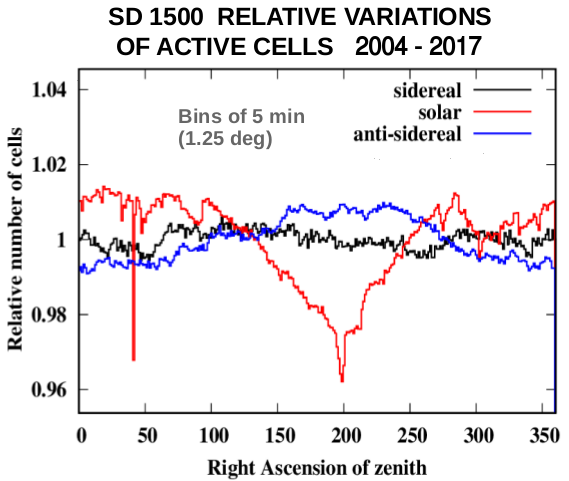
\includegraphics[width=0.5\linewidth]{pesos_referencia.png}  
              \caption{Valores de $\Delta N_{cell, k}$ en el rango 2004-2017 para distintas frecuencias obtenidas en el trabajo \cite{referencia_pesos}.}
              \label{fig:pesos_referencia}
        \end{figure}

       En la Fig.\ref{fig:pesos_ejemplo} se observa valores obtenidos de $\Delta N_{cell,k}$  con el código escrito para este trabajo, en función de la ascensión recta del cenit  para $L=288$ segmentos. Se analizó el conjunto de datos  utilizado para obtener los resultados la Fig.\ref{fig:pesos_referencia}, con el fin de validar dicho código. Los datos se analizaron desde el 1 de Enero del 2004 a las 00:00:00\,GMT  hasta el 1 de Enero del 2017 a las 00:00:00\,GMT. Se  observa que estos los resultados obtenidos son compatibles con la Fig.\ref{fig:pesos_referencia}
      

       \begin{figure}[H]
          \centering
              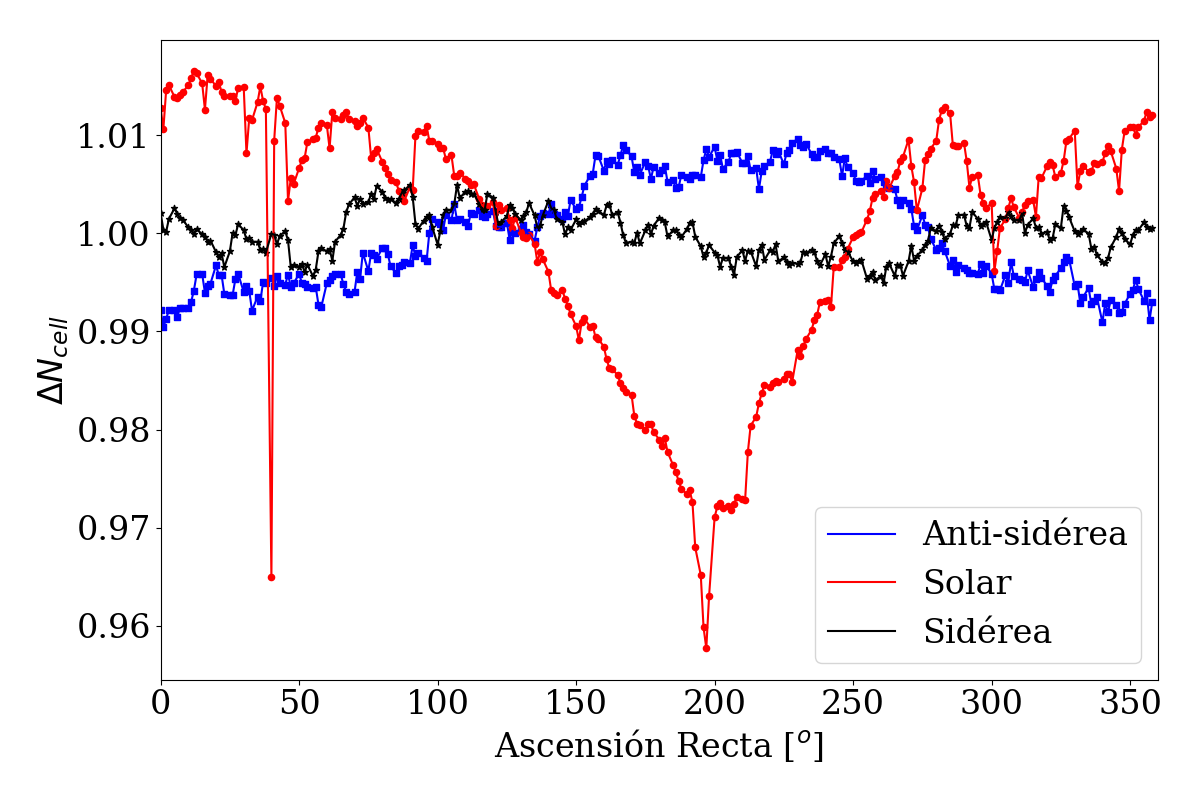
\includegraphics[width=0.75\linewidth]{weigths_2020.png}
              \caption{Valores de $\Delta N_{cell, k}$ en el rango 2004-2017 para distintas frecuencias utilizando el código escrito en este trabajo.}
              \label{fig:pesos_ejemplo}
        \end{figure}

      Para la frecuencia solar, se observa una variación apreciable con respecto al $1$. Esto se debe a un problema en la 

%En este trabajo se utilizó $L=288$ por razones discutidas anteriormente. 
    Para una representación fiel entre los registros de los hexágonos y los pesos de los eventos, se optó por clasificar los datos de los hexágonos en $288$ segmentos, donde cada segmento tiene un ancho de $1.25^o$. Esto es conveniente ya que la actualización del registro de hexágonos se realiza una vez  cada $5\,$min como se menciona en la sección \ref{hexagonos_rate}. Esta tasa de actualización es equivalente a decir que la adquisición se realiza cada vez que el cenit del observatorio barre  $1.25^o$ en ascensión recta sobre la esfera celeste.


%%%%%%%%%%%%%%%%%%%%%%%%%%%%%%%%%%%%%%%%%%%%%%%%%%%%%%%%%%%%%%%%%%%%%%%%%%%%%%%%%%%%%%%%%%%%%%%%%%%%%%
%hasta acá está chequeado

  \subsection{Cálculo de Rayleigh para una frecuencia dada} \label{rayleigh}

  La distribución en ascensión recta $\alpha$ del flujo de RCs $I(\alpha)$ que llega al arreglo principal puede caracterizarse por las amplitudes $r_k$ y fases $\phi_k$ de su expansión en serie de Fourier al $k-$ésimo orden. 

  \begin{equation}
    I(\alpha) = I_0 \bigg ( 1+ \sum^\infty_{k=1} r_k\cos{[k(\alpha - \phi_k)]} \bigg) = I_0 \bigg ( 1+ \sum^\infty_{k=1} a_k\cos{k\alpha} +  b_k\sin{k\alpha} \bigg ) 
  \end{equation}
  donde $a_k=r_k\cos\phi_k$ y $b_k=r_k\sin\phi_k$, y $I_0$ es el flujo medio. La distribución $I(\alpha)$ puede obtenerse a partir de la distribución de direcciones de arribo de los eventos observados. En este trabajo, se considera que todos los eventos $N$tienen una distribución uniforme en ascensión recta, es decir, $\nicefrac{dN}{d\alpha}= \sum^N_{i=1} \delta(\alpha - \alpha_i)$ \cite{taborda}. 

  Los análisis en ascensión recta están asociados a la frecuencia sidérea.  Para realizar el análisis de los eventos en cualquier frecuencia arbitraria, es necesario modificar $\alpha$ por $\tilde{\alpha}$. Esta nueva variable tiene la forma como se utiliza en el trabajo \cite{taborda}:
  \begin{equation}
    \tilde{\alpha} = 2\pi f_x t_i + \alpha_i - \alpha_i^0(t_i) \label{ra_mod}
  \end{equation}
  donde $f_x$ es el frecuencia arbitraria a estudiar, $t_i$ es el momento en que ocurrió el evento y $\alpha_i^0(t_i)$ es la ascensión recta del cenit del observatorio en el momento del evento. Si la frecuencia a analizar es la sidérea, el análisis con $\alpha$ y $\tilde{\alpha}$ arrojar los mismo parámetros $r_k$ y $\phi_k$.

  Por lo discutido en la sección anterior, puede existir una modulación debido a las variaciones de la exposición direccional.  Clasificando a los eventos mencionados en la sección \ref{specs} según el valor de la ascensión recta y considerando que todos los eventos tienen un peso uniforme de $w_i=1$, se dicen que los eventos fueron analizados \textit{sin pesos}, donde no consideramos la corrección de la exposición. En caso contrario, se habla de análisis \textit{con pesos} de los hexágonos  y estos pesos se calculan como se menciona en la sección anterior.

  Para realizar el análisis de frecuencias de los eventos, a primer orden en la expansión de Fourier, se siguen los siguientes pasos.

        \begin{enumerate}
        \item Fijando un rango de tiempo y un rango de energía en el cual se desea estudiar la anisotropía, se establece una frecuencia en particular $f$ a analizar.

        \item Con los eventos ya filtrados según el criterio de la sección \ref{filtro}, asigno cada evento $i$ un valor $h_i$, definida en la Ec.\ref{eq:h_horas}

        \item En caso de considerar los pesos de los hexágonos, para asignar el peso correspondiente al evento, se asocia a un segmento $k$, calculado en la sección \ref{peso_hexagonos}, mediante el valor de $h'_i$ definido en la Ec.\,\ref{eq:h_primado}. Luego, el peso asignado $w_i$  al evento $i$ es
        \begin{equation*}
           w_{i}= (\Delta N_{cell,k})^{-1}
        \end{equation*} 
        
        Caso contrario, se toman que todos los eventos tiene $w_i=1$.
        
        \item Para el análisis en frecuencias, a partir del valor de $h_i$ se asigna el ángulo $\tilde{\alpha}_i$ definida en la Ec.\ref{ra_mod}. La implementación en el código es de la siguiente manera:
        \begin{equation}
         \tilde{\alpha}_i = 2\pi \frac{h}{24} + \alpha_i -\alpha_{cenit,i}
        \end{equation}
        donde $\alpha_i$  representa la ascensión recta del evento y $\alpha_{cenit,i}$ la ascensión recta en el cenit del observatorio en el momento del evento. %A partir de este ángulo $\tilde{\alpha}_i$ se realiza en análisis en frecuencias.

        \item Para calcular los coeficientes de Fourier del primer armónico $a$ y $b$, se siguen los siguiente pasos:
        \begin{enumerate}
          \item Por cada evento  $i$ se calculan los siguientes valores:
          \begin{align}
             a_i' = {w_i}\cos\tilde{\alpha}_i \qquad
             b_i' = {w_i}\sin\tilde{\alpha}_i
         \end{align}
         \item Una vez que se obtuvieron los valores de $a_i'$ y $b_i'$ para todos los eventos en el rango de tiempo estudiado, se calculan los coeficientes definidos en el trabajo \cite{analisis_fourier} mediante:
         \begin{alignat}{3}
          \mathcal{N} &= \sum^{Eventos}_i w_i \\
            a &= \frac{2}{\mathcal{N}} \sum^{Eventos}_i a_i' \qquad
            b = \frac{2}{\mathcal{N}} \sum^{Eventos}_i b_i'  
         \end{alignat}
        \end{enumerate}
        \item Con los coeficientes es posible calcular la amplitud de la frecuencia estudiada $\tilde{r}$ y la fase $\phi$. Otros parámetros calculados para el análisis son la probabilidad $P(\tilde{r})$  y $r_{99}$. Cabe resaltar que el P99 depende solamente de los pesos de los eventos que se está estudiando. La interpretación  de este valor es cual es la probabilidad de tener una amplitud mayor como una fluctuación de una distribución isotrópica., y el valor de amplitud $r_{99}$ para que dicha probabilidad sea del $1$\%. 
        \begin{alignat}{3}
            \tilde{r} &= \sqrt{a^2 +b^2}                        \qquad &&   \phi&&= \arctan\frac{a}{b}\\
          P(\tilde{r})&= \exp(-\mathcal{N}\frac{\tilde{r}^2}{4})\qquad &&   r_{99}&&= \sqrt{\frac{-4\log(0.01)}{\mathcal{N}}}
        \end{alignat}

      \end{enumerate}

    Una forma de validar el código para el análisis de anisotropía es comparar los resultados del código con los obtenidos en otros trabajos \cite{taborda}. En la Fig.\ref{fig:sin_pesos_referencia} se muestra el análisis hecho sobre el mismo conjunto de eventos. Estos eventos fueron adquiridos con el disparo estándar desde el 1 de Enero del 2004 a las $00:00:00\,$GMT  hasta el 1 de Enero del 2017 a las $00:00:00\,$GMT. Se consideraron los eventos por encima de $8\,$EeV que además cumplan las condiciones dadas en la sección \ref{filtro}.  En esta figura que los resultados obtenidos en \cite{taborda} y con el código utilizado por este trabajo son indistinguibles. 

      \begin{figure}[H]
        \centering
        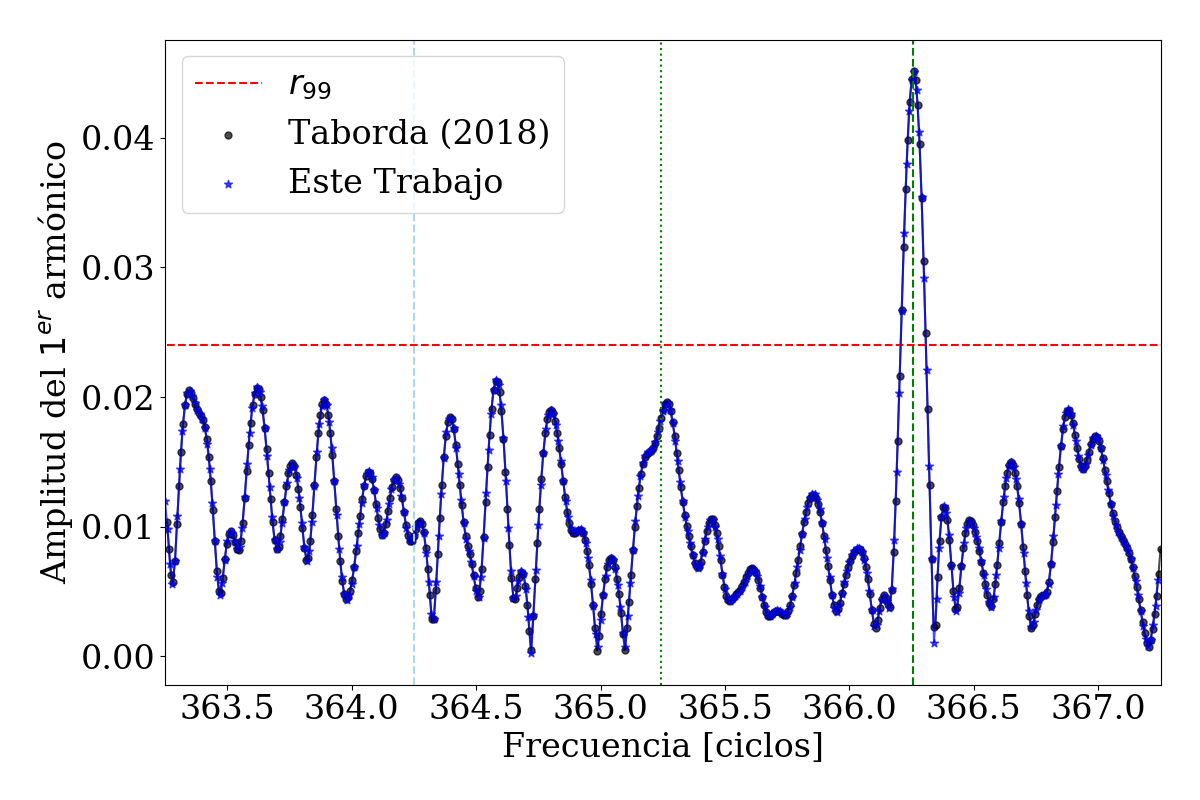
\includegraphics[width=0.75\linewidth]{sin_pesos_referencia_8_EeV.png}
        \caption{Comparación entre los análisis de anisotropía hechos para el mismo conjunto de datos, con el código de \cite{taborda} y con el código escrito para este trabajo.}
        \label{fig:sin_pesos_referencia}
      \end{figure}
